\documentclass[english, 12 pt]{report}
\usepackage[T1]{fontenc}
\usepackage[utf8]{luainputenc}
\usepackage{babel}
\usepackage[hidelinks, bookmarks]{hyperref}
\usepackage{geometry}
\geometry{verbose,tmargin=1cm,bmargin=3cm,lmargin=2cm,rmargin=2cm,headheight=3cm,headsep=1cm,footskip=1cm}
\setlength{\parindent}{0bp}
\usepackage{amsmath}
\usepackage{amssymb}
\usepackage{esint}
\usepackage{import}

\usepackage{graphicx}
\usepackage{placeins}
\raggedbottom
\usepackage{calc}
\usepackage{cancel}
\makeatletter
\usepackage{color}
\definecolor{shadecolor}{rgb}{0.105469, 0.613281, 1}
\usepackage{framed}
\usepackage{wrapfig}
\usepackage{bm}
\usepackage{ntheorem}

\usepackage{ragged2e}
\RaggedRight
\raggedbottom
\frenchspacing
\newcommand{\vsk}{\newline\vspace{11 pt}}
\newcommand{\vs}{\\ 
\includegraphics[]{lina} \\[5 pt]}
\begin{document}
	
\includegraphics[]{br1}
	\vs
	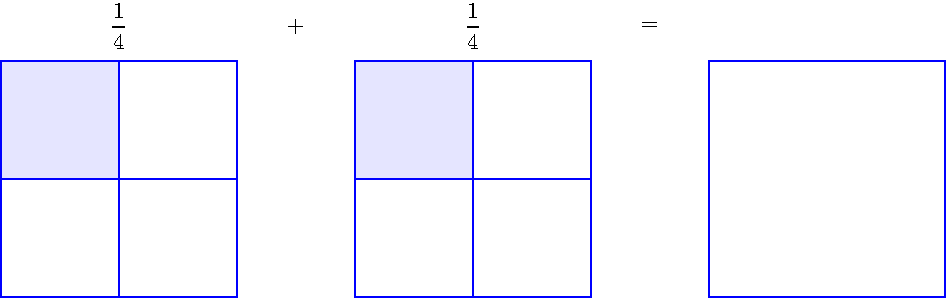
\includegraphics[]{br4}  \\[12 pt]
	Regel:\\ \vspace{5pt}
	$\qquad\qquad\displaystyle \frac{1}{4}\cdot2 =  $
	\vs
	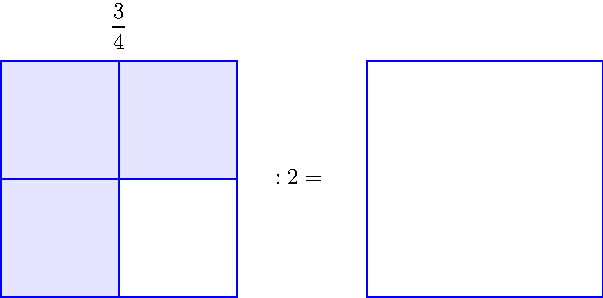
\includegraphics[]{br5b} \\[12 pt]
Regel:\\ \vspace{5pt}
$\qquad\qquad\displaystyle \frac{3}{4}:2 =  $	
	\vs
	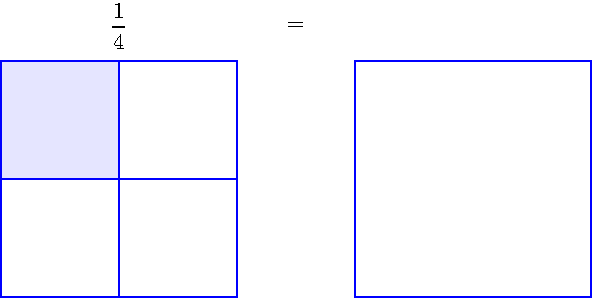
\includegraphics[]{br6}
	\vs
	
\includegraphics[]{br7}	
				
\end{document}
